% Sångtext till VN:s sångbok 2010.

% Denna fil kan användas som sådan, bara verserna,
% namnen och annan rådata behöver bytas ur fälten.
% Tecknet "%" markerar en kommentar som helt och 
% hållet ignoreras av programmet som läser filen.

\beginsong{Crambamboli}[ 		% Börja sången här
	by={},					% Författare
	sr={},					% Melodi
	index={När gud en gång den vackra världen skapade}]						% sång 



\beginverse*						% Börja vers
När Gud en gång den vackra världen skapade
så fann Han allting ganska gott.
Han tyckte dock att Adam borde
få något drickbart på sin lott.
Så satt han pricken över i
och skapade crambamboli,
cram-bim-bam-bamboli,
crambamboli!
\endverse							% Sluta vers

\beginverse*						% Börja vers
Napoleon, han var en tapper krigare
som du, som jag, som mången annan.
Och vet du vad om honom sades
var grunden till hans tapperhet?
Napoleon med sitt kompani
han drack ett glas crambamboli,
cram-bim-bam-bamboli,
crambamboli!
\endverse							% Sluta vers


\beginverse*						% Börja vers
Vill du som jag hos flickor/pojkar göra lycka?
Det kan gå bra, det kan gå galet.
Och vet: Det är ett vågat stycke
som fodrar ganska mycket mod.
Men jag kan sätta ett mot tre
att hjälpa skall crambamboli,
cram-bim-bam-bamboli,
crambamboli!
\endverse							% Sluta vers


\beginverse*						% Börja vers
Crambamboli, ja det är jordens härlighet
och himlens salighet, förvisso!
En härlig dryck för tjocka magar
och för den magre ganska gott.
All jordens sorg och tyranni
skall vika för crambamboli,
cram-bim-bam-bamboli,
crambamboli!
\endverse							% Sluta vers
\endsong							% Sluta sång

\begin{figure}[!b]
\begin{center}
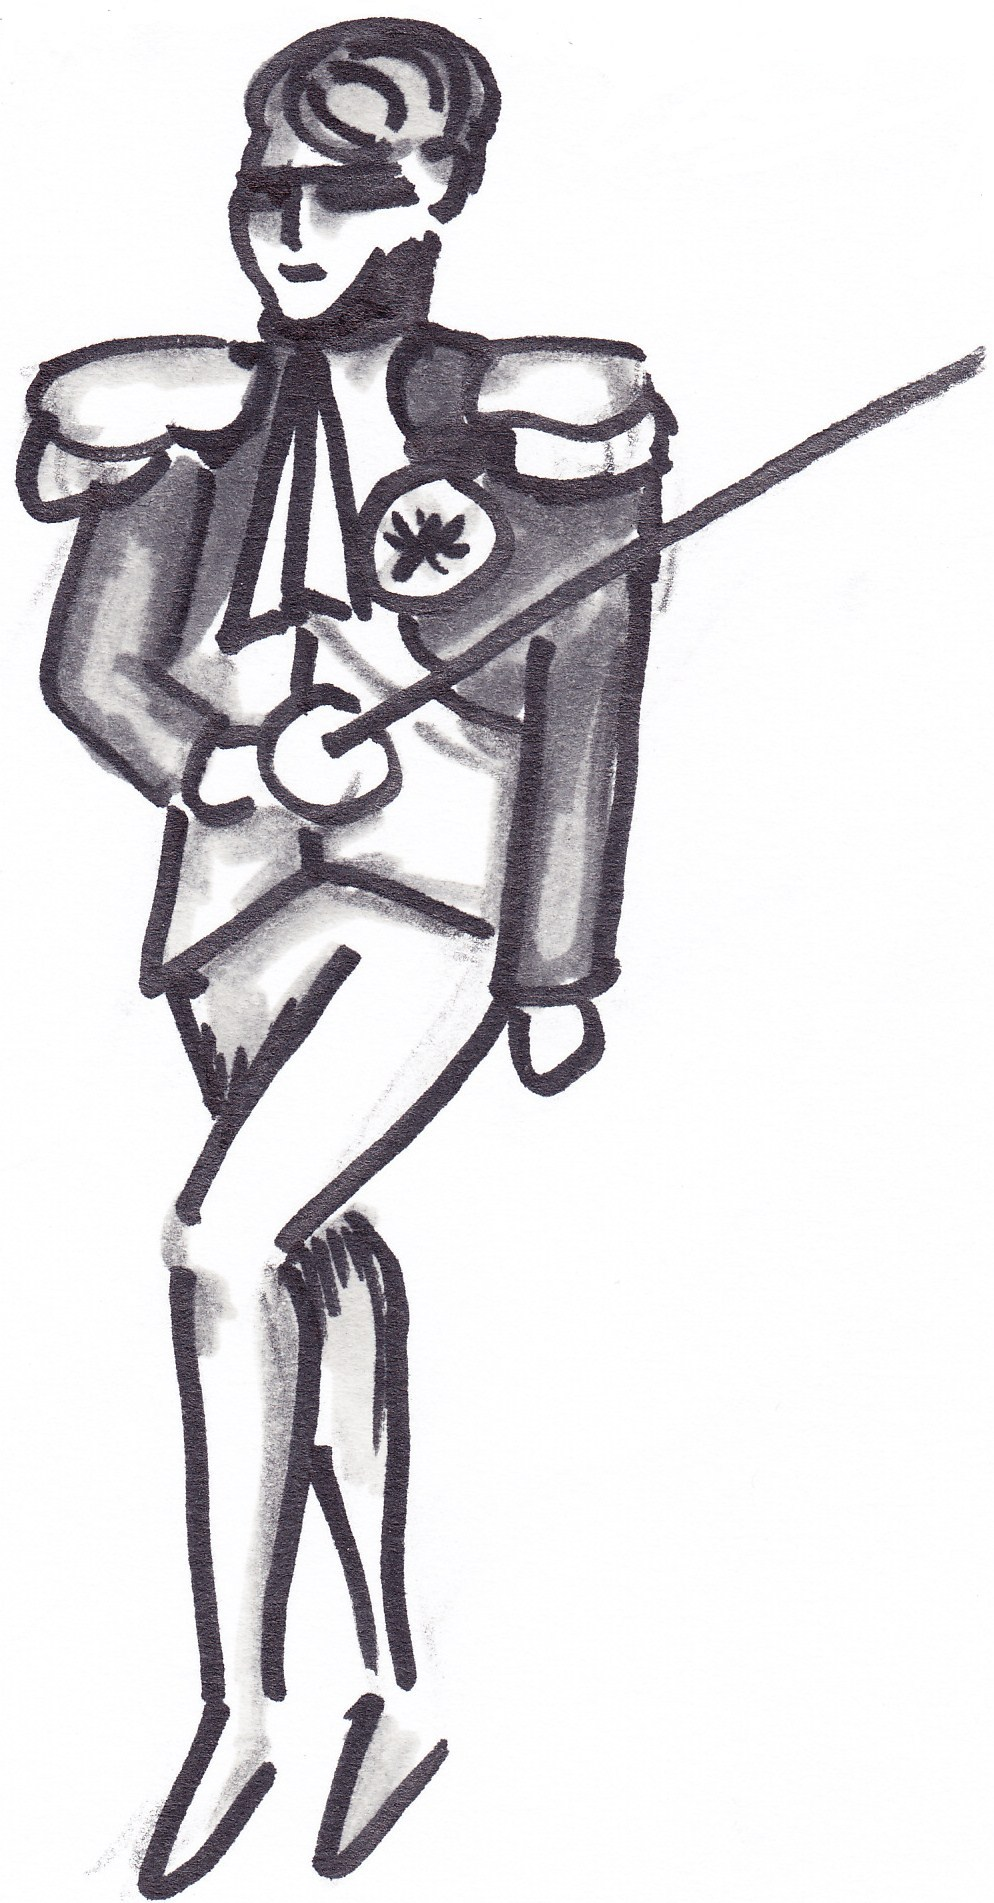
\includegraphics[scale=.5]{../bilder/crambamboli.jpg} 
\end{center}
\end{figure}